\section{Durchführung des Versuchs}
In Abbildung~\ref{fig:stm1} sehen wir das RTM, welches in der
folgenden Versuchsdurchführung verwendet wurde. Es handelt sich
um das Modell \textit{easyScan 2 STM, Version 1.6} welches von 
der Firma \textit{Nanoscience Instruments, Ink.} vertrieben wird.
Laut der Beschreibung des Herstellers 
bilden hunderte {easyScan 2 STMs} einen
\textit{unersetzlichen} Bestandteil in der Lehre von Physik,
Chemie und Materialwissenschaften, werden aber auch in der
Forschung und Entwicklung eingesetzt. Anwendung findet das RTM
in der Spektroskopie sowie in der Grundlagenforschung.
In unserem Versuch spielt das easyScan 2 STM insofern eine Rolle,
dass es ohne weitere Zwischeninstanzen direkt die gemessen
Abstände in ein Bild auf dem Computer sendet. Diese Bilder
enthalten schon alle für den Versuch notwendigen Informationen,
die Parameter können auch direkt von dem bereitgestellten Programm
konfiguriert werden. Der Wandel vom ersten RTM, in dem die Dämpfung
noch von Supraleitenden Magneten und einer Vakuumkammer hergestellt
werden musste, zum diesem Modell und diese Fortschritt kommt uns
in unserem FP zu Gute. Die Spezifikationen des Modells 
(Ausschnitt, entnommen aus dem beiliegendem Handbuch):\\
\noindent

\begin{tabular}{| l | p{7cm} |}
\hline
  Größe des Controllers, Gewicht: & 470x120x80 mm / 2.4 Kg\\ \hline
  Leistung & 90- 240 V~/ 30 W 50/60 Hz \\ \hline
  Rastergeschwindigkeit & Bis zu 60ms pro Linie mit 128 Datenpunkten  pro Linie \\ \hline
Rasterfläche & bis zu 2048x2048 Punkten \\ \hline 
Darstellungsmöglichkeiten: & Liniengraph, Farbplot und 3D Perspektive \\ \hline
Abbildungsmodi & Konstante Stromstärke (\textit{Constant Current}),
konstante Höhe (\textit{Constant Height}) \\ \hline
Maximale Auflösung in Z/ XY & 3pm/ 7.6pm \\ \hline
Maximaler Rasterumfang in Z/ XY & 200nm/ 500nm  \\ \hline
Maximale Probengröße & 10mm Durchmesser \\ \hline
Spitzenspannung & max. $\pm 10V$ in 5mV Schritten \\ \hline
\end{tabular}

\begin{figure}
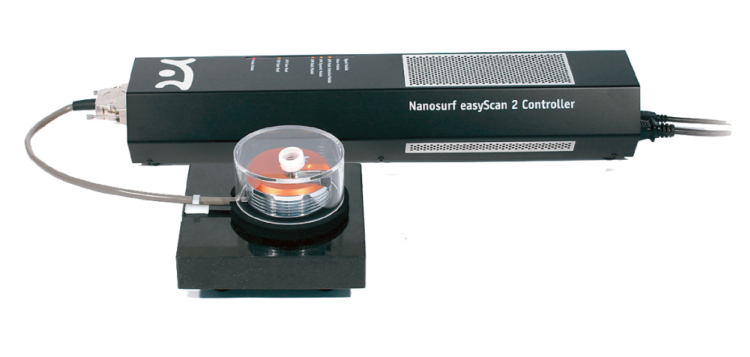
\includegraphics[width=14cm]{pics/stm1}
\caption{Photographie des verwendeten RTMs \textit{easyScan 2
STM Version 1.6} (entnommen aus Webseite des Herstellers)} 
 \label{fig:stm1}
\end{figure}

Da die Messaparatur für unseren Versuch schon aufgebaut worden
war und nicht modifiziert werden sollte, werden wir hier nicht
auf die einzelnen Komponenten des \textit{easy Scan 2 STM} Systems
eingehen, sondern nur die für unseren Versuch relevanten 
Bauteile beschreiben.
\subsection{Versuchsaufbau}
In Abbildung~\ref{fig:Rasterkopf} ist der Rasterkopf ds RTMs zu
sehen. Über den Probenhalter mit dazugehörigem Fixierungsmagneten
wird die Probe selbst angebracht; an den Spitzenhalter mit
Klammer die Spitze aus Platin-Iridiumdraht, 
welche wir für die Messungen selbst herstellt haben (siehe
Abbildung~\ref{fig:prepare_tip} und Abbildung~\ref{SEM_tip_picture}).
Der Probehalter stellt einen Zylinder dar, an dessen Kopf mithilfe
eines Magneten die Probe, welche im Idealfall auf einer dafür
passenden, ebenfalls magnetischen Schablone angebracht ist, 
befestigt wird, nachdem die Spitze angebracht wurde. 
Das Anbringen der Spitze erfolgt mit dafür passenden Zangen,
indem die Klammer angehoben, die Spitze eingelegt und mit
der Klammer fixiert wird.

\begin{figure}
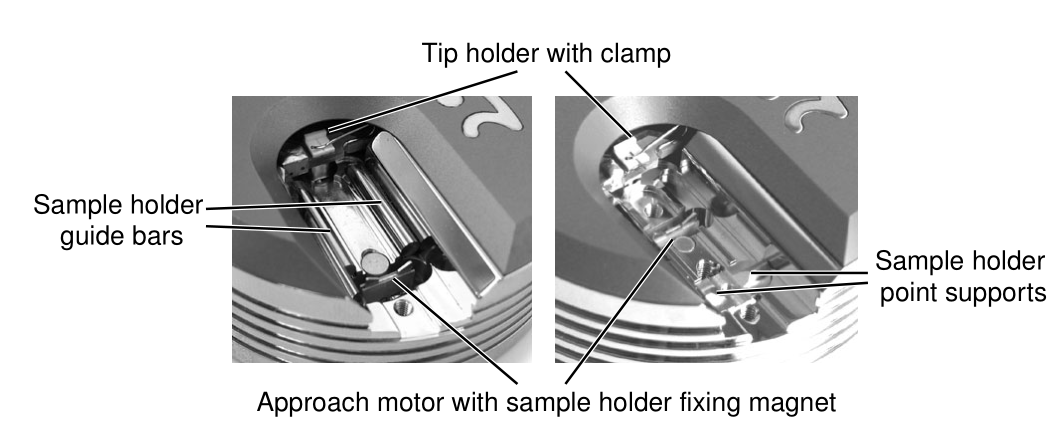
\includegraphics[width=14cm]{pics/rasterkopf}
\caption{Rasterkopf des RTMs \textit{easyScan 2
STM Version 1.6} (entnommen aus Webseite des Herstellers)
Zu sehen ist der Probenhalter (\textit{Sample holder}) mit dazu
gehörendem Annäherungsmotor (\textit{Approach motor} sowie
dem Fixierungsmagneten ({Fixing Magnet}), sowie dem Spitzenhalter
mit Klammer (\textit{Tip holder with clamp}). Die Funktionsweise
wird im Text beschrieben.}
 \label{fig:Rasterkopf}
\end{figure}

\begin{figure}
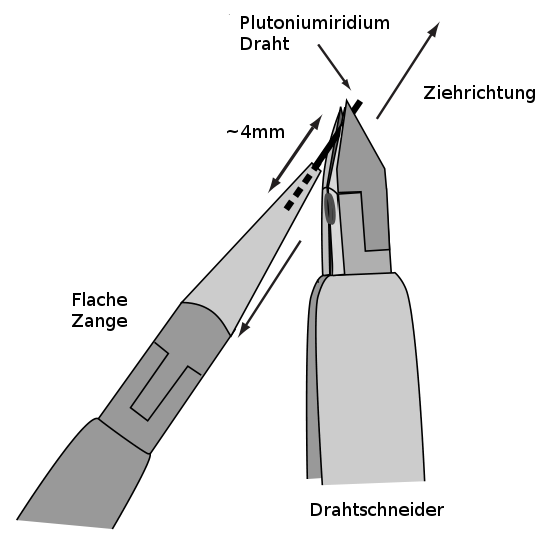
\includegraphics[width=10cm]{pics/prepare_tip2}
\caption{Vorbereitung des Drahtes. 1) Zunächst sollten die
zur Herstellung der Spitze notwendigen Werkzeuge mit Ethanol
gereinigt werden, von nun an sollte nur der Draht damit berührt 
werden. 2) Nun sollte der zu verknappende Draht mit den Zangen
gehalten werden, 3) dem Drahschneider umschlossen, aber nicht
abgezwickt, 4) in die angegebene Richtung \textbf{gezogen}, 5)
und endlich \textbf{abgerissen} werden, mit dem Ziel eine 
einatomige Spitze zu erzeugen (siehe Abbildung~\ref{fig:SEM_tip_picture})}
 \label{fig:prepare_tip}
\end{figure}

\begin{figure}
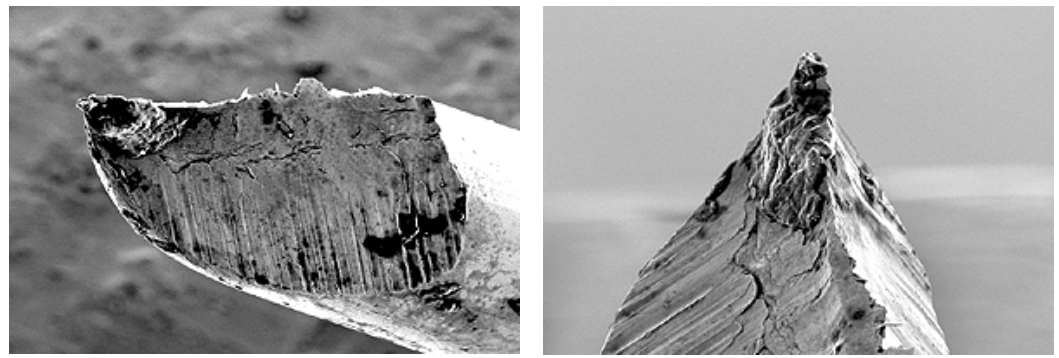
\includegraphics[width=10cm]{pics/SEM_tip_picture}
\caption{Das in Abbildung~\ref{fig:prepare_tip} beschriebene
Verfahren hat zum Ziel, eine möglichst präzise Spitze herzustellen.
Hier eine \textit{Scanning Electron Microskope} Abbildung
aus der Bedingungsanleitung des RTMs 
einer solchen hergestellen, idealen Spitze. Wie deutlich erkennbar
ist, verjüngt sich die Spitze nach oben und bietet so unter 
Umständen die Möglichkeit, eine einatomige Tunnelverbindung
mit der Probe einzugehen.}
 \label{fig:SEM_tip_picture}

\end{figure}
\subsection{Durchführung der Messungen}
Sobald die Spitze angebracht und die Probe eingeführt wurde, 
kann der Annäherungsprozess der Spitze zu der Probe beginnen. 
Zunächst kann manuell mit einer groben Steuerung die Spitze
(visuell) so nah wie möglich an die Probe herangebracht werden.
Dabei ist es von Vorteil, wenn diese schon zu Beginn recht nahe
aneinander liegen. Danach wird der automatische Annäherungsprozess
gestartet, der die Spitze solange mit einer jeweils eingestellten
Geschwindigkeit der Probe annähert, bis ein erster Tunnelstrom
zwischen der Probe und der Spitze fließen kann.  
Dieser Annäherungsversuch verfügt über verschiedene Modi:
\begin{itemize}
    \item \textbf{\textcolor{orange}{orange}}:
            Der Annäherungsversuch ist noch
            nicht abgeschlossen
    \item \textbf{\textcolor{red}{rot}}: 
            Der Annäherungsversuch ist in dem Sinne
            gescheitert, dass die Spitze mit der Probe kollidiert
            ist und womöglich Schaden erlitten hat. 
    \item \textbf{\textcolor{green}{grün}}: 
            Der Annäherungsversuch
            wurde ohne Fehlermeldungen
            abgeschlossen und ist vermutlich geglückt;
            der Tunnelstrom fließt wie vorgegeben.
\end{itemize}
